% Flowchart of one (per-level) timestep: hydro, then the radiation subcycle loop
% (QuokkaSimulation::advanceSingleTimestepAtLevel -> subcycleRadiationAtLevel, development @ 1e792e102).
% Build:  python figures/fig_flowchart.py plot   -> <figures>/fig_flowchart.pdf
% Drawn at its printed size (figure* width) so fonts match the paper's 10pt Computer Modern.
\documentclass[tikz,border=2pt]{standalone}
\usepackage{amsmath,amssymb}
\usetikzlibrary{calc,arrows.meta,backgrounds,shapes.geometric}

\newcommand{\chat}{\hat{c}}
\newcommand{\dtr}{\Delta t_{\rm rad}}
\newcommand{\R}{\mathsf{R}}
\newcommand{\V}{\mathsf{V}}
\newcommand{\T}{\mathcal{T}}
\newcommand{\Sg}{\mathcal{S}_g}
\newcommand{\Nlo}{N_{g,\rm lo}}

% Okabe-Ito hues, used as light tints
\definecolor{cHydro}{HTML}{999999}
\definecolor{cChem}{HTML}{E69F00}
\definecolor{cTrans}{HTML}{0072B2}
\definecolor{cImpl}{HTML}{009E73}
\definecolor{cLink}{HTML}{D55E00}
\definecolor{cTherm}{HTML}{CC79A7}

\begin{document}
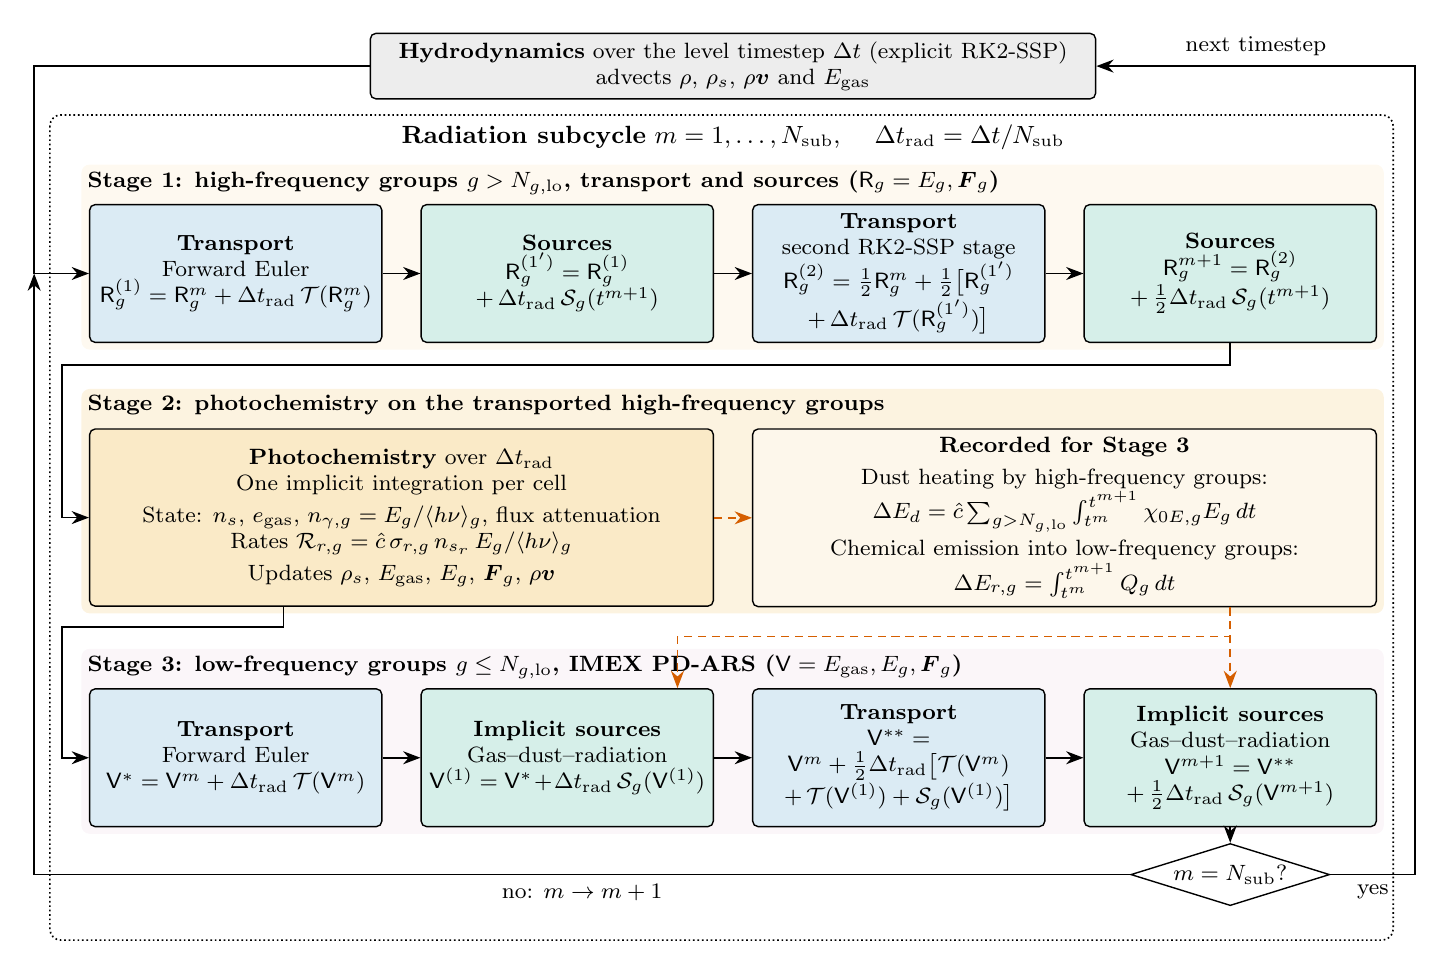
\begin{tikzpicture}[
	font=\footnotesize,
	>={Stealth[length=2.2mm]},
	box/.style={draw, rounded corners=2pt, align=flush center, inner sep=3pt, line width=0.5pt},
	hydro/.style={box, fill=cHydro!18, text width=9.0cm},
	cell/.style={box, anchor=north, text width=\boxW cm, minimum height=\boxH cm},
	trans/.style={cell, fill=cTrans!14},
	impl/.style={cell, fill=cImpl!16},
	photo/.style={box, anchor=north, fill=cChem!22, text width=\photoW cm, minimum height=\photoH cm},
	extra/.style={box, fill=cChem!8, text width=\photoW cm, minimum height=1.0cm},
	flow/.style={->, line width=0.6pt},
	link/.style={->, densely dashed, line width=0.6pt, cLink},
	lane/.style={draw=none, rounded corners=3pt},
	lanehead/.style={anchor=north west, font=\footnotesize\bfseries, inner sep=2pt},
]

% ---- horizontal layout (cm): 4 box columns, rails ----
\def\boxW{3.5}                      % box text width; outer width ~ \boxW + 0.21
\def\pitch{4.21}                    % column spacing (outer width + 0.5 gap)
\def\xA{2.71} \pgfmathsetmacro\xB{\xA+\pitch} \pgfmathsetmacro\xC{\xB+\pitch} \pgfmathsetmacro\xD{\xC+\pitch}
\pgfmathsetmacro\photoX{(\xA+\xB)/2} \pgfmathsetmacro\sideX{(\xC+\xD)/2}
\pgfmathsetmacro\photoW{\boxW+\pitch}
\def\laneL{0.75} \pgfmathsetmacro\laneR{\xD+\boxW/2+0.2}
\def\loopX{0.15} \def\retX{0.5}    % loop/hydro entry rail, row-return rail
\pgfmathsetmacro\frameR{\laneR+0.12} \pgfmathsetmacro\exitX{\laneR+0.4}

% ---- vertical layout (cm): lane tops ----
\def\boxH{1.75} \def\photoH{2.25}
\def\yA{-1.25} \def\yB{-4.1} \def\yC{-7.4}
\def\head{0.5}                      % lane header strip above the boxes

% ---- hydro ----
\node[hydro] (hydro) at ({(\xA+\xD)/2}, 0) {%
	\textbf{Hydrodynamics} over the level timestep $\Delta t$ (explicit RK2-SSP)\\
	advects $\rho$, $\rho_s$, $\rho\boldsymbol{v}$ and $E_{\rm gas}$};
\node[anchor=north, font=\small] (subtitle) at ({(\xA+\xD)/2}, -0.62) {%
	\textbf{Radiation subcycle} $m = 1,\dots,N_{\rm sub}$, \quad
	$\dtr = \Delta t/N_{\rm sub}$};

% ---- row A (Stage 1): high-frequency groups, explicit RK2-SSP transport + sources ----
\node[lanehead] (hA) at (\laneL, \yA) {Stage 1: high-frequency groups $g > \Nlo$, transport and sources ($\R_g = E_g, \boldsymbol{F}_g$)};
\node[trans] (A1) at (\xA, \yA-\head) {\textbf{Transport}\\ Forward Euler\\ $\R_g^{(1)} = \R_g^{m} + \dtr\,\T(\R_g^{m})$};
\node[impl]  (A2) at (\xB, \yA-\head) {\textbf{Sources}\\ $\R_g^{(1')} = \R_g^{(1)}$\\ $+\, \dtr\,\Sg(t^{m+1})$};
\node[trans] (A3) at (\xC, \yA-\head) {\textbf{Transport}\\ second RK2-SSP stage\\ $\R_g^{(2)} = \tfrac12\R_g^{m} + \tfrac12\big[\R_g^{(1')}$\\ $+\, \dtr\,\T(\R_g^{(1')})\big]$};
\node[impl]  (A4) at (\xD, \yA-\head) {\textbf{Sources}\\ $\R_g^{m+1} = \R_g^{(2)}$\\ $+\, \tfrac12\dtr\,\Sg(t^{m+1})$};

% ---- row B (Stage 2): photochemistry ----
\node[lanehead] (hB) at (\laneL, \yB) {Stage 2: photochemistry on the transported high-frequency groups};
\node[photo] (photo) at (\photoX, \yB-\head) {%
	\textbf{Photochemistry} over $\dtr$\\
	One implicit integration per cell\\[2pt]
	State: $n_s$, $e_{\rm gas}$, $n_{\gamma,g} = E_g/\langle h\nu\rangle_g$, flux attenuation\\
	Rates $\mathcal{R}_{r,g} = \chat\,\sigma_{r,g}\,n_{s_r}\,E_g/\langle h\nu\rangle_g$\\[2pt]
	Updates $\rho_s$, $E_{\rm gas}$, $E_g$, $\boldsymbol{F}_g$, $\rho\boldsymbol{v}$};
\node[extra, anchor=north, minimum height=\photoH cm] (qd) at (\sideX, \yB-\head) {%
	\textbf{Recorded for Stage 3}\\[2pt]
	Dust heating by high-frequency groups:\\
	$\Delta E_{d} = \chat \sum_{g>\Nlo} \int_{t^m}^{t^{m+1}} \chi_{0E,g} E_g\,dt$\\[2pt]
	Chemical emission into low-frequency groups:\\
	$\Delta E_{r,g} = \int_{t^m}^{t^{m+1}} Q_g\,dt$};

% ---- row C (Stage 3): low-frequency groups + gas, IMEX PD-ARS ----
\node[lanehead] (hC) at (\laneL, \yC) {Stage 3: low-frequency groups $g \le \Nlo$, IMEX PD-ARS ($\V = E_{\rm gas}, E_g, \boldsymbol{F}_g$)};
\node[trans] (C1) at (\xA, \yC-\head) {\textbf{Transport}\\ Forward Euler\\ $\V^{*} = \V^{m} + \dtr\,\T(\V^{m})$};
\node[impl]  (C2) at (\xB, \yC-\head) {\textbf{Implicit sources}\\ Gas--dust--radiation\\ $\V^{(1)} = \V^{*} + \dtr\,\Sg(\V^{(1)})$};
\node[trans] (C3) at (\xC, \yC-\head) {\textbf{Transport}\\ $\V^{**} = \V^{m} + \tfrac12\dtr\big[\T(\V^{m})$\\ $+\,\T(\V^{(1)}) + \Sg(\V^{(1)})\big]$};
\node[impl]  (C4) at (\xD, \yC-\head) {\textbf{Implicit sources}\\ Gas--dust--radiation\\ $\V^{m+1} = \V^{**}$\\ $+\, \tfrac12\dtr\,\Sg(\V^{m+1})$};

% ---- end-of-subcycle decision ----
\node[diamond, draw, aspect=3.2, inner sep=1pt, line width=0.5pt, fill=white] (dec)
	at ($(C4.south) + (0,-6mm)$) {$m = N_{\rm sub}$?};

% ---- main flow ----
\foreach \a/\b in {A1/A2, A2/A3, A3/A4, C1/C2, C2/C3, C3/C4}
	\draw[flow] (\a.east) -- (\b.west);
% row returns: A -> photochemistry -> C
\coordinate (gAB) at (0, {(\yA-\head-\boxH+\yB)/2});
\coordinate (gBC) at (0, {(\yB-\head-\photoH+\yC)/2});
\draw[flow] (A4.south) -- (A4.south |- gAB) -- (\retX, 0 |- gAB) |- (photo.west);
\draw[flow] ([xshift=-1.5cm]photo.south) -- ([xshift=-1.5cm]photo.south |- gBC) -- (\retX, 0 |- gBC) |- (C1.west);
\draw[flow] (C4.south) -- (dec.north);
% hydro -> first subcycle, and loop back
\draw[flow] (hydro.west) -| (\loopX, 0 |- A1.west) -- (A1.west);
\draw[flow] (dec.west) -- (\loopX, 0 |- dec.west) node[pos=0.5, below] {no: $m \to m+1$} -- (\loopX, 0 |- A1.west);
% exit
\draw[flow] (dec.east) -- (\exitX, 0 |- dec.east) node[midway, below] {yes} -- (\exitX, 0 |- hydro.east) -- (hydro.east)
	node[pos=0.5, above, rotate=0] {next timestep};

% ---- couplings produced by the photochemistry solve ----
\draw[link] (photo.east |- qd.west) -- (qd.west);
\coordinate (gQd) at (0, {(\yB-\head-\photoH+\yC)/2 - 0.12});
\draw[link] (qd.south -| C4.north) -- (C4.north);
\draw[link] (qd.south -| C4.north) |- ([xshift=1.4cm]C2.north |- gQd) -- ([xshift=1.4cm]C2.north);

% ---- background: subcycle frame and lanes ----
\begin{scope}[on background layer]
	\draw[line width=0.6pt, densely dotted, rounded corners=4pt]
		(\loopX+0.2, 0 |- subtitle.north) rectangle (\frameR, {\yC-\head-\boxH-1.45});
	\fill[lane, fill=cChem!6]  (\laneL, \yA) rectangle (\laneR, {\yA-\head-\boxH-0.1});
	\fill[lane, fill=cChem!12] (\laneL, \yB) rectangle (\laneR, {\yB-\head-\photoH-0.1});
	\fill[lane, fill=cTherm!7] (\laneL, \yC) rectangle (\laneR, {\yC-\head-\boxH-0.1});
\end{scope}

\end{tikzpicture}
\end{document}
